% Corrected MID trade-off scatter from rerun_mid_perscene.
% x = Cast_rel (lower is better); y = Chroma_err against MID pseudo-GT (lower is better).
\begin{figure}[t!]
  \centering
  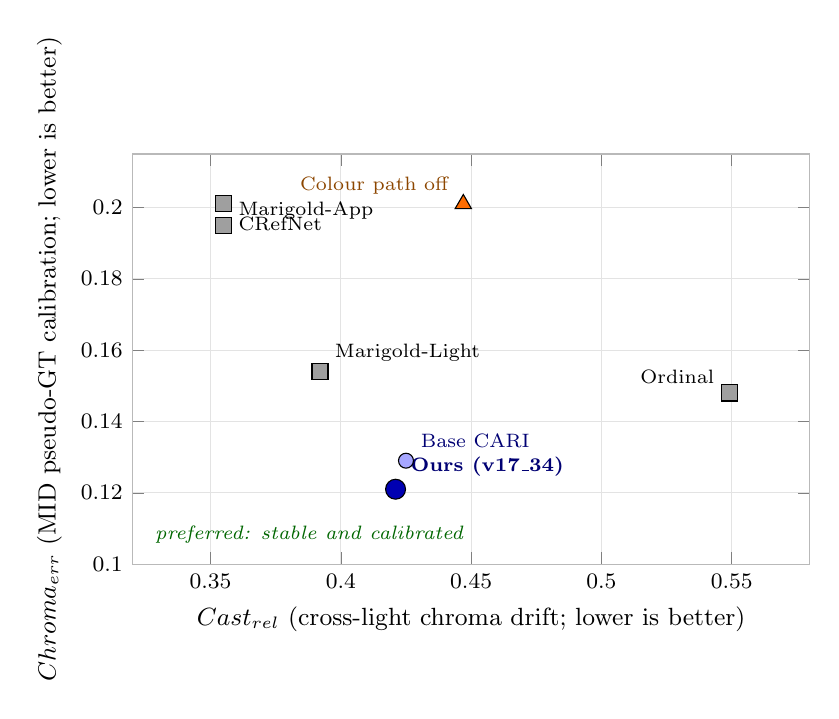
\begin{tikzpicture}
    \begin{axis}[
        width=0.84\textwidth, height=0.56\textwidth,
        xlabel={$\text{Cast}_{\text{rel}}$ (cross-light chroma drift; lower is better)},
        ylabel={$\text{Chroma}_{\text{err}}$ (MID pseudo-GT calibration; lower is better)},
        xlabel style={font=\small}, ylabel style={font=\small},
        tick label style={font=\footnotesize},
        xmin=0.32, xmax=0.58,
        ymin=0.10, ymax=0.215,
        grid=major,
        grid style={gray!22},
        axis line style={gray!55},
        clip=false,
      ]
      \node[anchor=south west, font=\scriptsize\itshape, text=green!40!black]
        at (axis cs:0.325,0.103) {preferred: stable and calibrated};

      \addplot[only marks, mark=*, mark size=3.6pt, draw=black, fill=blue!70!black]
        coordinates {(0.421,0.121)};
      \node[anchor=south west, font=\scriptsize\bfseries, blue!45!black]
        at (axis cs:0.423,0.122) {Ours (v17\_34)};

      \addplot[only marks, mark=*, mark size=2.7pt, draw=black, fill=blue!35]
        coordinates {(0.425,0.129)};
      \node[anchor=south west, font=\scriptsize, blue!45!black]
        at (axis cs:0.427,0.130) {Base CARI};

      \addplot[only marks, mark=triangle*, mark size=3.4pt, draw=black, fill=orange!85!red]
        coordinates {(0.447,0.201)};
      \node[anchor=south east, font=\scriptsize, orange!55!black]
        at (axis cs:0.445,0.201) {Colour path off};

      \addplot[only marks, mark=square*, mark size=2.9pt, draw=black, fill=gray!75]
        coordinates {(0.355,0.195) (0.392,0.154) (0.355,0.201) (0.549,0.148)};
      \node[anchor=south west, font=\scriptsize] at (axis cs:0.357,0.194) {Marigold-App};
      \node[anchor=south west, font=\scriptsize] at (axis cs:0.394,0.154) {Marigold-Light};
      \node[anchor=north west, font=\scriptsize] at (axis cs:0.357,0.200) {CRefNet};
      \node[anchor=south east, font=\scriptsize] at (axis cs:0.547,0.148) {Ordinal};
    \end{axis}
  \end{tikzpicture}
  \caption[MID constancy versus pseudo-GT chroma calibration.]{%
    Cross-light chroma stability against pseudo-GT chroma calibration on the
    30-scene MID test split. Lower is better on both axes. Marigold-App and
    CRefNet have lower drift but substantially higher calibration error; the
    selected model occupies a compromise region rather than winning either
    property universally. The companion spread diagnostic in
    \figref{fig:chroma_fidelity} shows whether low drift is accompanied by
    chroma collapse.
  }
  \label{fig:tradeoff}
\end{figure}
